% !TEX root = ../Coherence.tex

\section{Categorical coherence} 
\label{s:catoperads}

%%%%%%%%%%%%%%%%%%%%%%%%%%%%%%%%%%%%%
 
\subsection{Categorified non-symmetric operad}
\label{ss:def-catoperads}

Throughout this section we consider structures without units.
Unless otherwise stated, the adjective ``non-unital" will be implicitly assumed. 

\begin{definition} 
\label{def:catoperad}
A \defn{categorified non-symmetric operad} $\mathcal{P}$ is a collection $\left\{  \mathcal{P}(n)  \right\}_{n\in \mathbb{N}}$ of small categories equipped with bifunctors  
$$ \begin{array}{clll}
\circ_i&\colon& \mathcal{P}(n) \times
                    \mathcal{P}(k)
                    \longrightarrow \mathcal{P}(n+k-1) \ ,
                    & \text{for}\ 1 \leq i \leq n \ ,
\end{array}  $$
and for each $\kappa \in \mathcal{P}(m)$,  $\mu \in \mathcal{P}(n)$, $\nu \in \mathcal{P}(k)$, $1 \leq i \leq m$, $1 \leq j \leq n$ natural isomorphisms 
$$ \begin{array}{clll}
    \beta_{\kappa,\mu,\nu}&\colon& 
    (\kappa \circ_i \mu) \circ_{j+i-1} \nu  \overset{\cong}{\longrightarrow} \kappa \circ_i (\mu \circ_j \nu) \ , &  \\
    \theta_{\kappa,\nu,\mu}&\colon& 
    (\kappa \circ_i \nu) \circ_{j+k-1} \mu 
    \overset{\cong}{\longrightarrow} (\kappa \circ_j \mu) \circ_i \nu \ , & \text{when}\ i < j \ , 
\end{array}  $$
such that the following diagrams commute: the pentagonal \\
\begin{center}
\resizebox{\linewidth}{!}{
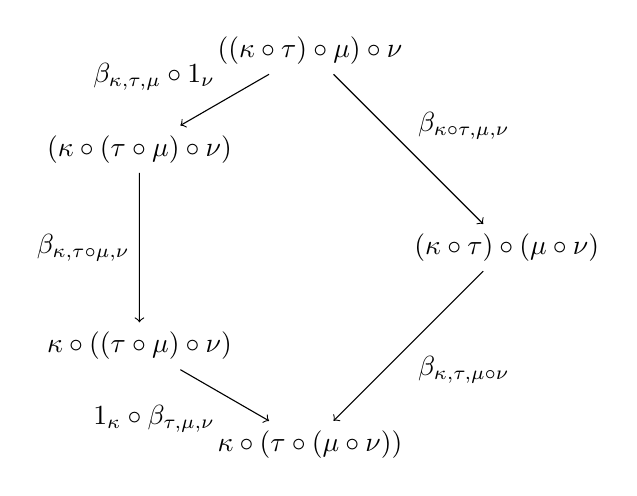
\begin{tikzpicture}[scale=2.5]
    \node (P1) at (0,1) {$((\kappa\circ\tau)\circ\mu)\circ\nu$};
    \node (P2) at (-0.866,0.5) {$(\kappa\circ(\tau\circ\mu)\circ\nu)$};
    \node (P3) at (-0.866,-0.5) {$\kappa\circ((\tau\circ\mu)\circ\nu)$};
    \node (P4) at (0,-1) {$\kappa\circ(\tau\circ(\mu\circ\nu))$};
    \node (P5) at (1,0) {$(\kappa\circ\tau)\circ(\mu\circ\nu)$} ;
    \draw[->] (P1)--(P2) node[midway,above left] {$\beta_{\kappa,\tau,\mu}\circ 1_\nu$};
    \draw[->] (P2)--(P3) node[midway,left] {$\beta_{\kappa,\tau\circ\mu,\nu}$};
    \draw[->] (P3)--(P4) node[midway,below left] {$1_\kappa \circ \beta_{\tau,\mu,\nu}$};
    \draw[->] (P1)--(P5) node[midway,above right] {$\beta_{\kappa\circ\tau,\mu,\nu}$};
    \draw[->] (P5)--(P4) node[midway,below right] {$\beta_{\kappa,\tau,\mu\circ\nu}$};
\end{tikzpicture} \quad 
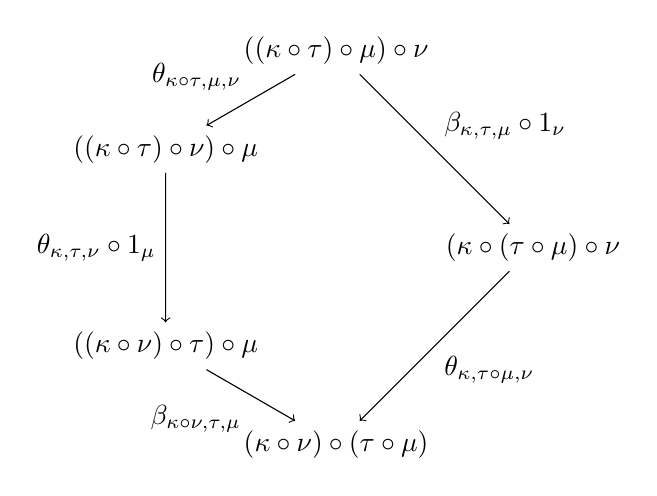
\begin{tikzpicture}[scale=2.5]
    \node (P1) at (0,1) {$((\kappa\circ\tau)\circ\mu)\circ\nu$};
    \node (P2) at (-0.866,0.5) {$((\kappa\circ\tau)\circ\nu)\circ\mu$};
    \node (P3) at (-0.866,-0.5) {$((\kappa\circ\nu)\circ\tau)\circ\mu$};
    \node (P4) at (0,-1) {$(\kappa\circ\nu)\circ(\tau\circ\mu)$};
    \node (P5) at (1,0) {$(\kappa\circ(\tau\circ\mu)\circ\nu$} ;
    \draw[->] (P1)--(P2) node[midway,above left] {$\theta_{\kappa\circ\tau,\mu,\nu}$};
    \draw[->] (P2)--(P3) node[midway,left] {$\theta_{\kappa,\tau,\nu}\circ 1_\mu$};
    \draw[->] (P3)--(P4) node[midway,below left] {$\beta_{\kappa\circ\nu,\tau,\mu}$};
    \draw[->] (P1)--(P5) node[midway,above right] {$\beta_{\kappa,\tau,\mu}\circ 1_\nu$};
    \draw[->] (P5)--(P4) node[midway,below right] {$\theta_{\kappa,\tau\circ\mu,\nu}$};
\end{tikzpicture} } \\
\end{center}

\begin{center}
\resizebox{0.5\linewidth}{!}{
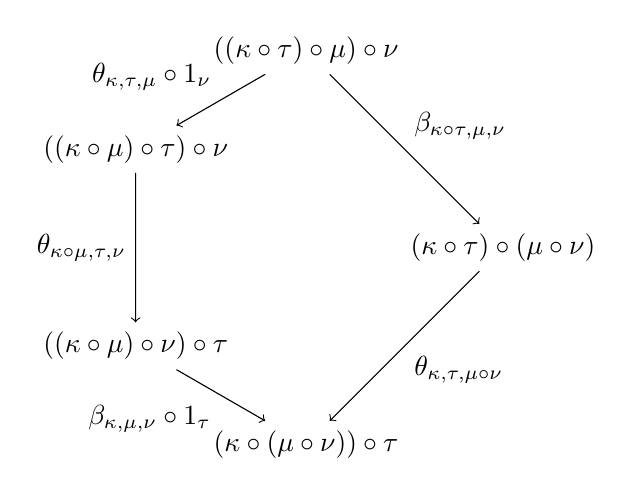
\begin{tikzpicture}[scale=2.5]
    \node (P1) at (0,1) {$((\kappa\circ\tau)\circ\mu)\circ\nu$};
    \node (P2) at (-0.866,0.5) {$((\kappa\circ\mu)\circ\tau)\circ\nu$};
    \node (P3) at (-0.866,-0.5) {$((\kappa\circ\mu)\circ\nu)\circ\tau$};
    \node (P4) at (0,-1) {$(\kappa\circ(\mu\circ\nu))\circ\tau$};
    \node (P5) at (1,0) {$(\kappa\circ\tau)\circ(\mu\circ\nu)$} ;
    \draw[->] (P1)--(P2) node[midway,above left] {$\theta_{\kappa,\tau,\mu}\circ 1_\nu$};
    \draw[->] (P2)--(P3) node[midway,left] {$\theta_{\kappa\circ\mu,\tau,\nu}$};
    \draw[->] (P3)--(P4) node[midway,below left] {$\beta_{\kappa,\mu,\nu}\circ 1_\tau$};
    \draw[->] (P1)--(P5) node[midway,above right] {$\beta_{\kappa\circ\tau,\mu,\nu}$};
    \draw[->] (P5)--(P4) node[midway,below right] {$\theta_{\kappa,\tau,\mu\circ\nu}$};
\end{tikzpicture}}
\end{center}

and hexagonal identities \\
\begin{center}
\resizebox{\linewidth}{!}{
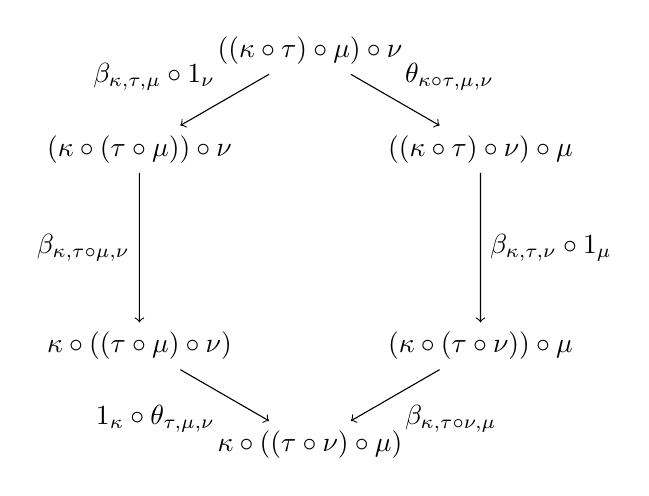
\begin{tikzpicture}[scale=2.5]
    \node (P1) at (0,1) {$((\kappa\circ\tau)\circ\mu)\circ\nu$};
    \node (P2) at (-0.866,0.5) {$(\kappa\circ(\tau\circ\mu))\circ\nu$};
    \node (P3) at (-0.866,-0.5) {$\kappa\circ((\tau\circ\mu)\circ\nu)$};
    \node (P4) at (0,-1) {$\kappa\circ((\tau\circ\nu)\circ\mu)$};
    \node (P5) at (0.866,0.5) {$((\kappa\circ\tau)\circ\nu)\circ\mu$} ;
    \node (P6) at (0.866,-0.5) {$(\kappa\circ(\tau\circ\nu))\circ\mu$};
    \draw[->] (P1)--(P2) node[midway,above left] {$\beta_{\kappa,\tau,\mu}\circ 1_\nu$};
    \draw[->] (P2)--(P3) node[midway,left] {$\beta_{\kappa,\tau\circ\mu,\nu}$};
    \draw[->] (P3)--(P4) node[midway,below left] {$1_\kappa \circ \theta_{\tau,\mu,\nu}$};
    \draw[->] (P1)--(P5) node[midway,above right] {$\theta_{\kappa\circ\tau,\mu,\nu}$};
    \draw[->] (P5)--(P6) node[midway,right] {$\beta_{\kappa,\tau,\nu}\circ 1_\mu$};
    \draw[->] (P6)--(P4) node[midway,below right] {$\beta_{\kappa,\tau\circ\nu,\mu}$};
\end{tikzpicture} \quad \quad
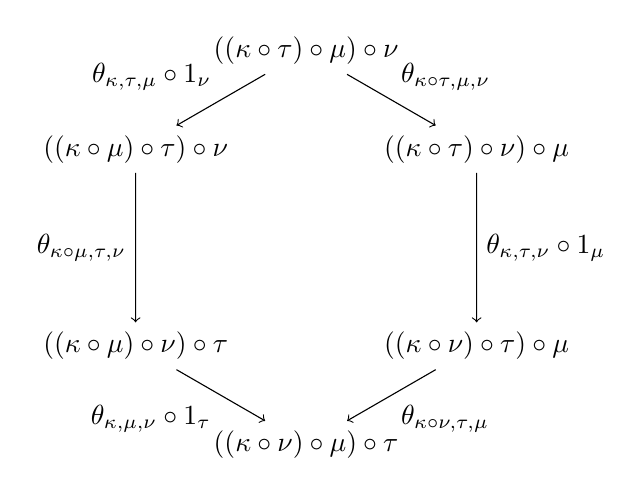
\begin{tikzpicture}[scale=2.5]
    \node (P1) at (0,1) {$((\kappa\circ\tau)\circ\mu)\circ\nu$};
    \node (P2) at (-0.866,0.5) {$((\kappa\circ\mu)\circ\tau)\circ\nu$};
    \node (P3) at (-0.866,-0.5) {$((\kappa\circ\mu)\circ\nu)\circ\tau$};
    \node (P4) at (0,-1) {$((\kappa\circ\nu)\circ\mu)\circ\tau$};
    \node (P5) at (0.866,0.5) {$((\kappa\circ\tau)\circ\nu)\circ\mu$} ;
    \node (P6) at (0.866,-0.5) {$((\kappa\circ\nu)\circ\tau)\circ\mu$};
    \draw[->] (P1)--(P2) node[midway,above left] {$\theta_{\kappa,\tau,\mu}\circ 1_\nu$};
    \draw[->] (P2)--(P3) node[midway,left] {$\theta_{\kappa\circ\mu,\tau,\nu}$};
    \draw[->] (P3)--(P4) node[midway,below left] {$\theta_{\kappa,\mu,\nu}\circ 1_\tau$};
    \draw[->] (P1)--(P5) node[midway,above right] {$\theta_{\kappa\circ\tau,\mu,\nu}$};
    \draw[->] (P5)--(P6) node[midway,right] {$\theta_{\kappa,\tau,\nu}\circ 1_\mu$};
    \draw[->] (P6)--(P4) node[midway,below right] {$\theta_{\kappa\circ\nu,\tau,\mu}$};
\end{tikzpicture}  } \quad \ .
\end{center}
\end{definition}
The diagrams above hold for all instances of composable $\beta$ and $\theta$; these depend on the indices $i,j,k$, which are omitted for the sake of readability. 
Observe that a categorified non-symmetric operad concentrated in arity $1$ is a non-symmetric monoidal category.

\correction{As explained in \cref{prop:bijection-nestings} below}, one can picture an object $\mu \in \mathcal{P}(n)$ as a planar tree with one vertex decorated by $\mu$, $n$ leaves and one root (a \defn{corolla}). 
The $\circ_i$ bifunctors then correspond to the operation of \defn{grafting} a corolla on top of another.
Iterated applications of the $\circ_i$ can be visualized as fully nested planar trees, with vertices decorated by objects of $\mathcal{P}$, see \cref{fig:treeandnesting}. 
\correction{A \defn{nesting} of a planar tree is a collection of subtrees (\defn{nests}) which are either included in one another or disjoint. 
A nesting is \defn{full} if its number of nests is maximal, equal to the number of internal edges of the tree \cite[Def.~2.2]{laplante-anfossiDiagonalOperahedra2022a}.}

\begin{figure}[h!]
\centering
\resizebox{0.4\linewidth}{!}{
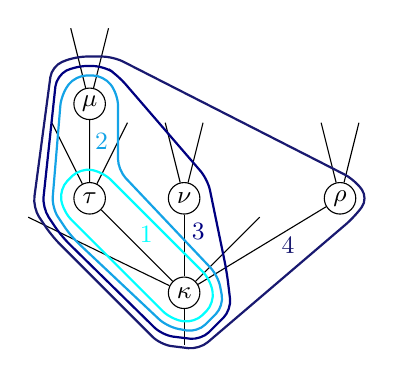
\begin{tikzpicture}[scale=1.2]
        \node (E)[circle,draw=black,minimum size=4mm,inner sep=0.1mm] at (-0,0) {\small $\kappa$};
        \node (F) [circle,draw=black,minimum size=4mm,inner sep=0.1mm] at (-1,1) {\small $\tau$};
        \node (A) [circle,draw=black,minimum size=4mm,inner sep=0.1mm] at (-1,2) {\small $\mu$};
        \node (q) [circle,draw=black,minimum size=4mm,inner sep=0.1mm] at (0,1) {\small $\nu$};
        \node (r) [circle,draw=black,minimum size=4mm,inner sep=0.1mm] at (1.65,1) {\small $\rho$};
        \node (x) [circle,draw=none,minimum size=4mm,inner sep=0.1mm] at (-0.4,0.62) {\color{Cyan} \small $1$};
        \node (y) [circle,draw=none,minimum size=4mm,inner sep=0.1mm] at (-0.875,1.6) {\color{Cerulean} \small $2$};
        \node (u) [circle,draw=none,minimum size=4mm,inner sep=0.1mm] at (0.15,0.65) {\color{NavyBlue} \small $3$};
        \node (v) [circle,draw=none,minimum size=4mm,inner sep=0.1mm] at (1.1,0.5) {\color{MidnightBlue} \small $4$};
        \draw[-] (0.8,0.8) -- (E)--(-1.65,0.8); 
        \draw[-] (-1.2,2.8) -- (A)--(-0.8,2.8); 
        \draw[-] (-0.2,1.8) -- (q)--(0.2,1.8);   
        \draw[-] (1.85,1.8) -- (r)--(1.45,1.8); 
        \draw[-] (E)--(0,-0.55); 
        \draw[-] (-1.4,1.8) -- (F)--(-0.6,1.8);   
        \draw[-] (E)--(F) node {};
        \draw[-] (E)--(q) node  {};
        \draw[-] (E)--(r) node {};
        \draw[-] (F)--(A) node {};
        \draw [Cyan,rounded corners,thick] (0.11,-0.32) -- (-0.14,-0.28) -- (-1.28,0.86) -- (-1.32,1.1) --  (-1.1,1.32) -- (-0.86,1.28) -- (0.28,0.14) -- (0.32,-0.11) -- cycle;
        \draw [Cerulean,rounded corners,thick] (0.14,-0.42) -- (-0.18,-0.36) -- (-1.2,0.6) -- (-1.4,0.9) -- (-1.3,2.1) -- (-1.15,2.3) -- (-0.85,2.3) -- (-0.7,2.1) --  (-0.7,1.3) -- (0.36,0.18) -- (0.42,-0.14) -- cycle;
        \draw [NavyBlue,rounded corners,thick] (0.18,-0.5) -- (-0.23,-0.45) -- (-1.3,0.6) -- (-1.5,0.9) --  (-1.35,2.3) --  (-1.15,2.4) --  (-0.85,2.4) --  (-0.7,2.3) --  (.25,1.2) -- (0.45,0.23) -- (0.5,-0.18) -- cycle;
        \draw [MidnightBlue,rounded corners,thick] (0.16,-0.6) -- (-0.25,-0.55) -- (-1.4,0.6) -- (-1.6,0.9) --  (-1.4,2.4) --  (-1.15,2.5) --  (-0.75,2.5) --  (1.8,1.2) --  (1.95,1) --  (1.8,0.8) -- cycle;
\end{tikzpicture} }
\caption{A fully nested planar tree.}
\label{fig:treeandnesting}
\end{figure} 

The $\beta$ and $\theta$ arrows correspond to the sequential and parallel axioms of an operad, and relate the two possible ways of \correction{fully} nesting a tree with $3$ vertices, see \cref{fig:betatheta}. 
Moreover, there is then one coherence diagram (pentagon or hexagon) for every planar tree with $4$ vertices, see \cref{fig:planar4trees}.

\begin{figure}[h!]
\begin{center}
\resizebox{0.25\linewidth}{!}{
\quad
\begin{tikzpicture}
    \node (t3)[circle,draw=black,minimum size=4mm,inner sep=0.1mm] at (0,0) {\small $\kappa$};
    \node (t2) [circle,draw=black,minimum size=4mm,inner sep=0.1mm] at (0,1) {\small $\mu$};
    \node (t1) [circle,draw=black,minimum size=4mm,inner sep=0.1mm] at (0,2) {\small $\nu$};  
    \draw[-] (t3)--(t2) node {};
    \draw[-] (t2)--(t1) node {};
    \draw [Plum,rounded corners,thick] (-0.15+2,0.7) -- (-0.3+2,0.9) -- (-0.3+2,2.1) -- (-0.15+2,2.3) -- (0.15+2,2.3) -- (0.3+2,2.1) -- (0.3+2,0.9) -- (0.15+2,0.7) -- cycle;

    \node (B) at (1,1) {$\overset{\beta}{\longrightarrow}$};

    \node (b3)[circle,draw=black,minimum size=4mm,inner sep=0.1mm] at (2,0) {\small $\kappa$};
    \node (b2) [circle,draw=black,minimum size=4mm,inner sep=0.1mm] at (2,1) {\small $\mu$};
    \node (b1) [circle,draw=black,minimum size=4mm,inner sep=0.1mm] at (2,2) {\small $\nu$};  
    \draw[-] (b3)--(b2) node {};
    \draw[-] (b2)--(b1) node {};
    \draw [Plum,rounded corners,thick] (1.85-2,-0.3) -- (1.7-2,-.1) -- (1.7-2,1.1) -- (1.85-2,1.3) -- (2.15-2,1.3) -- (2.3-2,1.1) -- (2.3-2,-.1) -- (2.15-2,-.3) -- cycle;
\end{tikzpicture}} \quad\quad \raisebox{2.75em}{}\quad\quad 
\resizebox{0.4\linewidth}{!}{
\raisebox{1em}{\begin{tikzpicture}
    \node (t3)[circle,draw=black,minimum size=4mm,inner sep=0.1mm] at (0,0) {\small $\kappa$};
    \node (t2) [circle,draw=black,minimum size=4mm,inner sep=0.1mm] at (0.71,0.71) {\small $\mu$};
    \node (t1) [circle,draw=black,minimum size=4mm,inner sep=0.1mm] at (-0.71,0.71) {\small $\nu$};  
    \draw[-] (t3)--(t1) node {};
    \draw[-] (t2)--(t3) node {};
    \draw [Plum,rounded corners,thick] (0.11,-0.32) -- (-0.14,-0.28) -- (-0.99,0.57) -- (-1.03,0.81) -- (-0.81,1.03) -- (-0.57,0.99)  -- (0.28,0.14) -- (0.32,-0.11) -- cycle;

    \node (B) at (1.5,0.5) {$\overset{\theta}{\longrightarrow}$};

    \node (b3)[circle,draw=black,minimum size=4mm,inner sep=0.1mm] at (3,0) {\small $\kappa$};
    \node (b2) [circle,draw=black,minimum size=4mm,inner sep=0.1mm] at (3+0.71,0.71) {\small $\mu$};
    \node (b1) [circle,draw=black,minimum size=4mm,inner sep=0.1mm] at (3-0.71,0.71) {\small $\nu$};  
    \draw[-] (b3)--(b1) node {};
    \draw[-] (b2)--(b3) node {};
    \draw [Plum,rounded corners,thick] (3-0.32,-0.11) -- (3-0.28,0.14) -- (3+0.57,0.99) -- (3+0.81,1.03) -- (3+1.03,0.81) -- (3+0.99,0.57) -- (3+0.14,-0.28) -- (3-0.11,-0.32) -- cycle;
\end{tikzpicture}}} \raisebox{2.75em}{} 
\end{center} 
\caption{The $\beta$ and $\theta$ isomorphisms defining a categorified non-symmetric operad.}
\label{fig:betatheta}
\end{figure}

\begin{figure}[h!]
\centering 
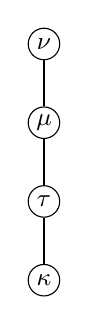
\begin{tikzpicture}
    \node (t3)[circle,draw=black,minimum size=4mm,inner sep=0.1mm] at (0,0) {\small $\kappa$};
    \node (t2) [circle,draw=black,minimum size=4mm,inner sep=0.1mm] at (0,1) {\small $\tau$};
    \node (t1) [circle,draw=black,minimum size=4mm,inner sep=0.1mm] at (0,2) {\small $\mu$};  
    \node (t4) [circle,draw=black,minimum size=4mm,inner sep=0.1mm] at (0,3) {\small $\nu$};  
    \draw[-] (t4)--(t1) node {};
    \draw[-] (t3)--(t2) node {};
    \draw[-] (t2)--(t1) node {};
\end{tikzpicture}
\quad \quad
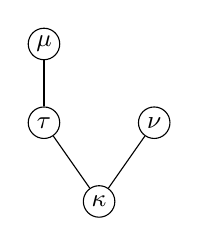
\begin{tikzpicture}
    \node (t3)[circle,draw=black,minimum size=4mm,inner sep=0.1mm] at (0,0) {\small $\kappa$};
    \node (t2) [circle,draw=black,minimum size=4mm,inner sep=0.1mm] at (-0.7,1) {\small $\tau$};
    \node (t1) [circle,draw=black,minimum size=4mm,inner sep=0.1mm] at (-0.7,2) {\small $\mu$};  
    \node (t4) [circle,draw=black,minimum size=4mm,inner sep=0.1mm] at (0.7,1) {\small $\nu$};  
    \draw[-] (t4)--(t3) node {};
    \draw[-] (t3)--(t2) node {};
    \draw[-] (t2)--(t1) node {};
\end{tikzpicture}
\quad \quad
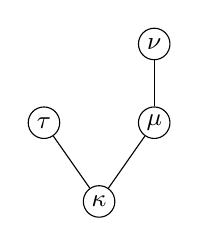
\begin{tikzpicture}
    \node (t3)[circle,draw=black,minimum size=4mm,inner sep=0.1mm] at (0,0) {\small $\kappa$};
    \node (t2) [circle,draw=black,minimum size=4mm,inner sep=0.1mm] at (-0.7,1) {\small $\tau$};
    \node (t1) [circle,draw=black,minimum size=4mm,inner sep=0.1mm] at (0.7,1) {\small $\mu$};  
    \node (t4) [circle,draw=black,minimum size=4mm,inner sep=0.1mm] at (0.7,2) {\small $\nu$};  
    \draw[-] (t4)--(t1) node {};
    \draw[-] (t3)--(t1) node {};
    \draw[-] (t2)--(t3) node {};
\end{tikzpicture}
\quad \quad
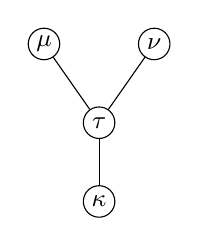
\begin{tikzpicture}
    \node (t3)[circle,draw=black,minimum size=4mm,inner sep=0.1mm] at (0,0) {\small $\kappa$};
    \node (t2) [circle,draw=black,minimum size=4mm,inner sep=0.1mm] at (0,1) {\small $\tau$};
    \node (t1) [circle,draw=black,minimum size=4mm,inner sep=0.1mm] at (-0.7,2) {\small $\mu$};  
    \node (t4) [circle,draw=black,minimum size=4mm,inner sep=0.1mm] at (0.7,2) {\small $\nu$};  
    \draw[-] (t4)--(t2) node {};
    \draw[-] (t3)--(t2) node {};
    \draw[-] (t2)--(t1) node {};
\end{tikzpicture}
\quad \quad
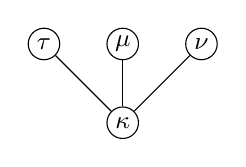
\begin{tikzpicture}
    \node (t3)[circle,draw=black,minimum size=4mm,inner sep=0.1mm] at (0,0) {\small $\kappa$};
    \node (t2) [circle,draw=black,minimum size=4mm,inner sep=0.1mm] at (-1,1) {\small $\tau$};
    \node (t1) [circle,draw=black,minimum size=4mm,inner sep=0.1mm] at (0,1) {\small $\mu$};  
    \node (t4) [circle,draw=black,minimum size=4mm,inner sep=0.1mm] at (1,1) {\small $\nu$};  
    \draw[-] (t4)--(t3) node {};
    \draw[-] (t3)--(t2) node {};
    \draw[-] (t3)--(t1) node {};
\end{tikzpicture}
\caption{The five planar trees with four vertices, giving rise to the pentagonal (first three) and hexagonal (last two) identites.}
\label{fig:planar4trees}
\end{figure}

\begin{rem}
\label{rem:DPLA}
K. Do{\v s}en and Z. Petri{\'c} introduced in \cite[Sec.~12]{DP15} the notion of weak Cat-operad.
Despite looking different at first sight, the two notions are in fact equivalent.
The crucial observation is the following: the $\theta$-isomorphisms of Do{\v s}en--Petri{\'c} comprise both the isomorphisms~$\theta$ in \cref{def:catoperad} and their inverses $\theta^{-1}$.
Therefore, there are only two pentagonal coherence diagrams in the definition of a weak Cat-operad, the equations ($\beta$ $pent_e$) and ($\beta\theta 2_e$) of \cite[Section 9]{DP15}.
The set of diagrams of the form ($\beta$ $pent_e$) is the same as the set of diagrams which arises from the first pentagon in \cref{def:catoperad}, while the set of diagrams of the form ($\beta\theta 2_e$) is partitioned into the sets of diagrams which arise from the second and third pentagons in \cref{def:catoperad}.

We will give in \cref{thm:coherence-operahedra} two topological proofs of coherence for categorified non-symmetric operads.
A benefit of our presentation is that, adopting the oriented approach (see the second proof of \cref{thm:coherence-operahedra}), we get a proof of coherence where $\beta$ and $\theta$ are both treated as rewriting rules, in contrast with the proof in \cite{DP15}, which proceeds in two stages, much like in Mac Lane's proof of coherence for symmetric monoidal categories (see~\cref{MacLane-Kapranov-Simple}): first get rid of $\beta$ (rewriting), then deal with $\theta$. 
\end{rem}

\begin{definition}
    A \defn{strong morphism} of categorified non-symmetric operads $F: \mathcal{P} \to \mathcal{Q}$ is a collection of functors $F_n : \mathcal{P}(n) \to \mathcal{Q}(n)$ together with natural isomorphisms $$ \gamma_{\kappa,\mu}: F_{m-1+n}(\kappa \circ_i \mu) \overset{\cong}{\longrightarrow} F_m(\kappa) \circ_i F_n(\mu) $$ such that the following diagrams commute:
    \begin{center}
    \resizebox{\linewidth}{!}{
    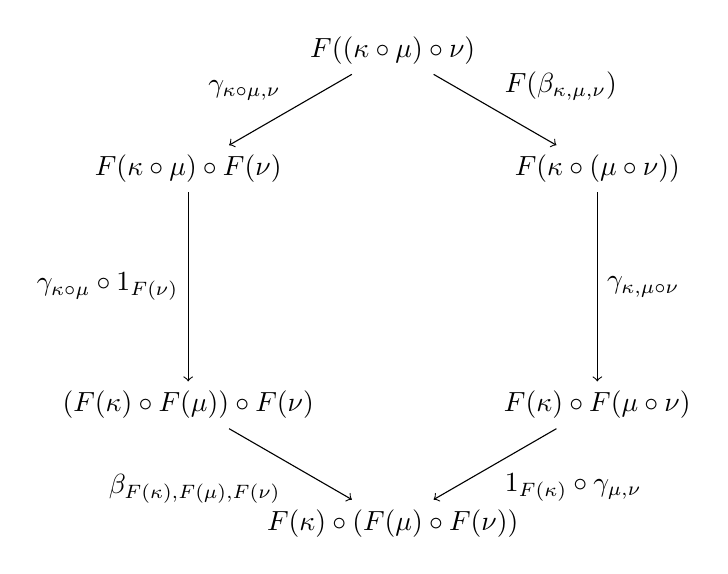
\begin{tikzpicture}[scale=3]
        \node (P1) at (0,1) {$F((\kappa\circ\mu)\circ\nu)$};
        \node (P2) at (-0.866,0.5) {$F(\kappa\circ\mu)\circ F(\nu)$};
        \node (P3) at (-0.866,-0.5) {$(F(\kappa)\circ F(\mu))\circ F(\nu)$};
        \node (P4) at (0,-1) {$F(\kappa)\circ(F(\mu)\circ F(\nu))$};
        \node (P5) at (0.866,0.5) {$F(\kappa\circ(\mu\circ\nu))$} ;
        \node (P6) at (0.866,-0.5) {$F(\kappa)\circ F(\mu\circ\nu)$};
        \draw[->] (P1)--(P2) node[midway,above left] {$\gamma_{\kappa\circ\mu,\nu}$};
        \draw[->] (P2)--(P3) node[midway,left] {$\gamma_{\kappa\circ\mu}\circ 1_{F(\nu)}$};
        \draw[->] (P3)--(P4) node[midway,below left] {$\beta_{F(\kappa),F(\mu),F(\nu)}$};
        \draw[->] (P1)--(P5) node[midway,above right] {$F(\beta_{\kappa,\mu,\nu})$};
        \draw[->] (P5)--(P6) node[midway,right] {$\gamma_{\kappa,\mu\circ\nu}$};
        \draw[->] (P6)--(P4) node[midway,below right] {$1_{F(\kappa)}\circ\gamma_{\mu,\nu}$};
    \end{tikzpicture}  \quad \quad
    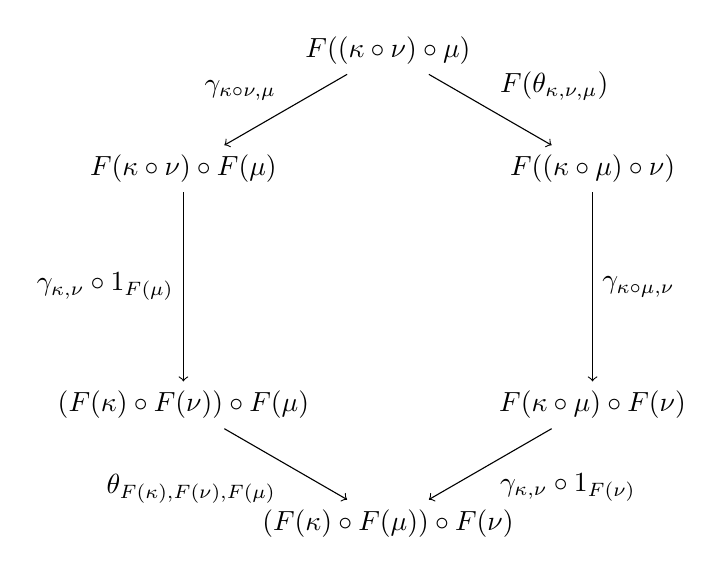
\begin{tikzpicture}[scale=3]
        \node (P1) at (0,1) {$F((\kappa\circ\nu)\circ\mu)$};
        \node (P2) at (-0.866,0.5) {$F(\kappa\circ\nu)\circ F(\mu)$};
        \node (P3) at (-0.866,-0.5) {$(F(\kappa)\circ F(\nu))\circ F(\mu)$};
        \node (P4) at (0,-1) {$(F(\kappa)\circ F(\mu))\circ F(\nu)$};
        \node (P5) at (0.866,0.5) {$F((\kappa\circ\mu)\circ\nu)$} ;
        \node (P6) at (0.866,-0.5) {$F(\kappa\circ\mu)\circ F(\nu)$};
        \draw[->] (P1)--(P2) node[midway,above left] {$\gamma_{\kappa\circ\nu,\mu}$};
        \draw[->] (P2)--(P3) node[midway,left] {$\gamma_{\kappa,\nu}\circ 1_{F(\mu)}$};
        \draw[->] (P3)--(P4) node[midway,below left] {$\theta_{F(\kappa),F(\nu),F(\mu)}$};
        \draw[->] (P1)--(P5) node[midway,above right] {$F(\theta_{\kappa,\nu,\mu})$};
        \draw[->] (P5)--(P6) node[midway,right] {$\gamma_{\kappa\circ\mu,\nu}$};
        \draw[->] (P6)--(P4) node[midway,below right] {$\gamma_{\kappa,\nu}\circ 1_{F(\nu)}$};
    \end{tikzpicture}  } \quad \ .
\end{center}
    It is said to be \defn{strict} if the natural isomorphisms are identities. 
\end{definition}

Once again, the diagrams above hold for all instances of $\beta$ and $\theta$ arrows, and we have omitted the $(i,j,k)$-indices for readability. 
Observe that a strong (resp. strict) morphism between categorified non-symmetric operads concentrated in arity $1$ is a strong (resp. strict) monoidal functor between non-symmetric monoidal categories. 

%%%%%%%%%%%%%%%%%%%%%%%%%%%%%%%%%%%%%%%%%%%%%%%

\subsection{Coherence for categorified non-symmetric operads}
\label{ss:coherence-catoperads}

We now aim at the coherence theorem for categorified non-symmetric operads.
In order to state the theorem, we construct the free non-symmetric categorified operad on a family of sets $S=\{S_n\}_{n \geq 1}$.
We define a family of categories~$\mathcal{S}=\{\mathcal{S}_n\}_{n \geq 1}$ whose objects are given by the following rules:
\begin{enumerate}
    \item if $a \in S_n$, then $a$ is an object of $\mathcal{S}_n$;
    \item if $t_1 \in \mathcal{S}_m$ and $t_2 \in \mathcal{S}_n$, then $t_1 \circ_i t_2$ is an object of $\mathcal{S}_{m-1+n}$, for any $1 \leq i \leq m$.
\end{enumerate}
If an object $t_1$ is in $\mathcal{S}_n$, we say that $t_1$ has \defn{arity} $n$. 
Now we define a set $M$ of \defn{basic morphisms} $\beta: (t_1 \circ_i t_2) \circ_{j+i-1} t_3 \leftrightarrow t_1 \circ_i (t_2 \circ_j t_3) : \beta^{-1}$ for every $t_1 \in \mathcal{S}_m, t_2 \in \mathcal{S}_n, t_3 \in \mathcal{S}_k$, $1 \leq i \leq m$ and $1 \leq j \leq n$, and $\theta: (t_1 \circ_i t_3) \circ_{j-1+k} t_2 \leftrightarrow (t_1 \circ_j t_2) \circ_i t_3 : \theta^{-1}$ whenever $i<j$.
We then define the \defn{generating morphisms} of the family $\mathcal{S}$ by the following rules:
\begin{enumerate}
    \item if $\phi \in M$, then $\phi$ is a generating morphism of $\mathcal{S}$; 
    \item if $\phi : t_1 \to t_2$ is a generating morphism in $\mathcal{S}$, and $t_3 \in \mathcal{S}$, then $\phi \circ_i \id : t_1 \circ_i t_3 \to t_2 \circ_i t_3$ and $\id \circ_j \phi : t_3 \circ_j t_1 \to t_3 \circ_j t_2$ are \correction{generating} morphisms, for any $i$ (resp. $j$) between~$1$ and the arity of $t_1$ (resp. $t_3$).
\end{enumerate}
Note that by construction, for every morphism $\phi : t_1 \to t_2$, the objects $t_1$ and $t_2$ have the same arity, and we say that $\phi$ has this \defn{arity}. 
We then define $\mathcal{S}_n$ as the free category over all generating morphisms of arity $n$. 
This finishes the construction of our family $\mathcal{S}$ of categories.

\begin{definition}
    We denote by $\mathcal{F}(S)$ the quotient of the family of categories $\mathcal{S}$ by localization (inverting the $\beta$ and $\theta$ morphisms), the axioms of bifunctors for the $\circ_i$, \correction{the naturality conditions for $\beta$ and $\theta$}, and the coherence diagrams (pentagons and hexagons) defining a categorified non-symmetric operad. 
\end{definition}

We obtain that $\mathcal{F}(S)$ is the free categorified non-symmetric operad on $S$. 
That is, for any categorified non-symmetric operad $\mathcal{P}$, and for any family of functions $\rho_n : S_n \to \obj(\mathcal{P}(n))$, there is a unique \emph{strict} morphism of non-symmetric categorified operads $\mathcal{F}(S) \to \mathcal{P}$ which extends $\rho=\{\rho_n\}_{n\geq 1}$. 
By precomposing it with the quotient map $\mathcal{S} \to \mathcal{F}(S)$, we get a levelwise functor $\extu{-}:\mathcal{S} \to \mathcal{P}$.

\begin{thm}[Coherence theorem]
\label{thm:coherence-operahedra}
    For any categorified non-symmetric operad $\mathcal{P}$, for any family of functions $\rho : S \to \obj(\mathcal{P})$, and for any two parallel morphisms $\phi_1,\phi_2: t_1 \to t_2$ in~$\mathcal{S}$, we have $\extu{\phi_1}=\extu{\phi_2}$.
\end{thm}

\correction{
In order to prove this \cref{thm:coherence-operahedra}, we need to first recall the construction of the \defn{operahedra}, a family of polytopes whose faces are in bijection with the set of all nestings of a planar tree.
We refer to \cite[Sec.~2]{laplante-anfossiDiagonalOperahedra2022a} for details, see also \cite[Sec.~13]{DP15} and \cite{curienSyntacticAspectsHypergraph2019a}.
Given a planar tree $t$ with $n$ internal edges, and a full nesting $\mathcal{N}$ of $t$, one associates a point~$M(t,\mathcal{N}) \in \R^n$ via a simple algorithm which is due to Jean-Louis Loday \cite[Sec.~2.2]{laplante-anfossiDiagonalOperahedra2022a}.  
The \defn{operahedron}~$P_t \subset \R^n$ is the convex hull of the points $M(t,\mathcal{N})$, for all maximal nestings $\mathcal{N}$ of $t$.
It has dimension $n-1$. 
One then shows that the poset of nestings of~$t$, ordered by reverse inclusion, is isomorphic to the poset of faces of~$P_t$ \cite[Prop.~2.15]{laplante-anfossiDiagonalOperahedra2022a}. 
The dimension of a face is given by $n$ minus the number of nests in the corresponding nesting of $t$.}

\correction{
    Reading a planar tree $t$ from the leaves to the root defines a family of \defn{incoming edges} and one \defn{outgoing edge} at each vertex of $t$.
    Given the family of sets $S$ and a planar tree $t$, we say that a decoration of the vertices of $t$ by elements of $S$ is \defn{admissible} if at every vertex the number of incoming edges is equal to the arity of the element of $S$ decorating it. 
Now, let us consider the collection $\mathcal{O}(S)$ of polytopes with one copy of the operahedron~$P_t$ for each admissible decoration of the planar tree $t$ by elements of $S$. 
\begin{samepage}
    \begin{proposition}
        \label{prop:bijection-nestings}
            There are bijections between
            \begin{enumerate}
                \item objects of $\calS$ and vertices of the operahedra in $\mathcal{O}(S)$,
                \item generating morphisms of $\calS$ and edges of the operahedra in $\mathcal{O}(S)$,
                \item bifunctoriality, naturality and coherence diagrams and $2$-faces of the operahedra in~$\mathcal{O}(S)$.
            \end{enumerate}
        \end{proposition}
\end{samepage}
\begin{proof}
To each element $a$ of $S_n$, we associate a planar corolla with $n$ leaves and vertex decorated by $a$. 
Then, we identify $a \circ_i b$ with the planar tree obtained from grafting the corolla decorated by $b$ at the $i$th leaf of the corolla decorated by $a$.
Continuing in this fashion, and remembering the order in which we graft the corollas, we obtain all possible fully nested planar trees with vertices decorated by elements of $S$ (\cref{fig:treeandnesting}).
A generating morphism $f$ in $\mathcal{S}$ is an application of one of the associativity rules~$\beta$ or~$\theta$ to a fully nested tree $t$, moving only one nest (\cref{fig:betatheta}). 
If $t$ has $n$ internal edges, forgetting the nest that has been moved gives a nesting of $t$ with $n-1$ nests.
We associate to $f$ the edge of the operahedron $P_t$ in $\mathcal{O}(S)$ labeled by this nesting, see \cite[Def.~2.8 \& Prop.~3.11]{laplante-anfossiDiagonalOperahedra2022a}.
It remains to consider all the possible diagrams one can obtain by applying two generating morphisms to a given fully nested tree $t$ with $n$ internal edges. 
These arise from moving two different nests in the same fully nested tree. 
Starting by moving one or the other of these $2$ nests, one faces two types of situations:
\begin{itemize}
    \item[(A1)] If the two nests are disjoint, one obtains a bifunctoriality square,
    \item[(A2)] If the two nests are nested, but do not share the same root, one obtains a naturality square,
    \item[(B)] If the two nests are nested and share the same root, one obtains either a pentagon or an hexagon as in \cref{def:catoperad}.
\end{itemize}
To such a diagram, we associate the $2$-face of the operahedron~$P_t$ in $\mathcal{O}(S)$ corresponding to the nesting of $t$ obtained by forgetting the two nests that have been moved along the edges.
We refer to \cite[Sec.~2]{CLA24} for a more detailed analysis of the $2$-faces.  
\end{proof}
\begin{rem}
    The fact that every possible choice of initial moves gives rise to a $2$-face amounts to the fact that the operahedron $P_t$ is a \emph{simple} polytope \cite[Sec.~9]{DP-HP}.
    As \cref{l:simple-local-diagrams} shows, this property garantees the correspondence between geometric and rewriting-theoretic proofs of coherence, see \cite{CLA24} for more details on the latter.
\end{rem}
The conceptual origin of the bijections of \cref{prop:bijection-nestings} is the fact that the combinatorics of the faces of the operahedra correspond exactly to the monad of trees \cite[Sec.~5.6.1]{LodayVallette12}.
Or, said differently, it lies in the fact that the operahedra encode (via the cellular chains functor) the minimal resolution of the colored symmetric operad whose algebras are non-unital non-symmetric operads, see \cite{VanDerLaan03} and \cite[Sec.~4.1]{laplante-anfossiDiagonalOperahedra2022a}.}

\correction{We are now ready to prove \cref{thm:coherence-operahedra}, using either our non-oriented or oriented topological coherence results for polytopes.}
\begin{proof}[Proof of {\cref{thm:coherence-operahedra}}]
    \correction{From Point (2) in \cref{prop:bijection-nestings}, we have that} the morphisms of~$\mathcal{S}$ are in bijection with combinatorial paths on the operahedra of $\mathcal{O}(S)$.
Two parallel morphisms in~$\mathcal{S}$ thus define two parallel combinatorial paths on some operahedron $P_t$ in $\mathcal{O}(S)$. 
Since an operahedron $P_t$ is simply connected, \cref{thm:top-coherence} implies that these two combinatorial paths are combinatorially homotopic. 
By \correction{Point (3) in \cref{prop:bijection-nestings}} the $2$-faces of the operahedra are exactly either a bifunctoriality or naturality square, a pentagon or an hexagon (witnessing a coherence condition) as in \cref{def:catoperad}.
\correction{
Therefore, two parallel morphisms $\phi_1,\phi_2$ in $\mathcal{S}$ are equal in the quotient $\mathcal{F}(S)$, and thus their images $\extu{\phi_1},\extu{\phi_2}$ are also equal in $\mathcal{P}$.} 
\end{proof}

\begin{proof}[Second proof of {\cref{thm:coherence-operahedra}}]
    Alternatively, since the operahedra are polytopes, one can use \cref{prop:polytopes} and \cref{p:second-proof}. 
    As shown in \cite[Prop.~3.11]{laplante-anfossiDiagonalOperahedra2022a}, choosing a generic vector $\vec v$ which has strictly decreasing coordinates gives the orientations of the diagrams given in \cref{def:catoperad} on the $2$-faces.
    One then obtains a topological proof of coherence which \correction{follows closely} the original proof of Mac Lane \cite[Thm.~3.1]{MacLane63}, suitably generalized to categorified operads. 
\end{proof}
   
Following \cref{rem:DPLA}, we have that \cref{thm:coherence-operahedra} gives an alternative, more economical proof of coherence for weak Cat-operads \cite[Prop.~14.2]{DP15}.
Incidentally, it gives an alternative input to the proof of coherence for cyclic symmetric categorified operads \cite{curienCategorifiedCyclicOperads2020}.

Restricting the theorem above to non-symmetric operads concentrated in arity $1$, the category $\mathcal{F}(S)$ becomes the free non-symmetric monoidal category on $S$, and we get the following corollary. 

\begin{corollary}[Mac Lane coherence theorem for non-symmetric monoidal categories]
\label{cor:MacLane}
    For any non-symmetric monoidal category $\mathcal{C}$, for any function $\rho : S \to \obj(\mathcal{C})$, and for any two parallel morphisms $\phi_1,\phi_2: t_1 \to t_2$ in $\mathcal{S}$, we have $\extu{\phi_1}=\extu{\phi_2}$.
\end{corollary}

\begin{rem}
    \correction{
    As mentioned at the end of \cref{ss:abstract-rewriting}, the rewriting systems obtained on the vertices of the operahedra by choosing a generic vector with strictly decreasing coordinates are in fact \emph{term} rewriting systems.
    The faces of type (B) in Point (3) of \cref{prop:bijection-nestings} (the coherence conditions) correspond precisely to the \emph{critical pairs} of these rewriting systems, see \cite[Sec.~3.4]{CLA24}.
    Moreover, the associated posets on fully nested planar trees have recently been shown to be lattices \cite{DefanSack24}.}
\end{rem}




